\documentclass[
	fontsize=12pt,           % Leitlinien sprechen von Schriftgröße 12.
	paper=A4,
	twoside=false,
	listof=totoc,            % Tabellen- und Abbildungsverzeichnis ins Inhaltsverzeichnis
	bibliography=totoc,      % Literaturverzeichnis ins Inhaltsverzeichnis aufnehmen
	titlepage,               % Titlepage-Umgebung anstatt \maketitle
	headsepline,             % horizontale Linie unter Kolumnentitel
	abstract,              % Überschrift einschalten, Abstract muss in {abstract}-Umgebung stehen
]{scrreprt}                  % Verwendung von KOMA-Report
\usepackage[utf8]{inputenc}  % UTF8 Encoding einschalten
\usepackage[ngerman]{babel}  % Neue deutsche Rechtschreibung
\usepackage[T1]{fontenc}     % Ausgabe von westeuropäischen Zeichen (auch Umlaute)
\usepackage{microtype}       % Trennung von Wörtern wird besser umgesetzt
\usepackage{lmodern}         % Nicht-gerasterte Schriftarten (bei MikTeX erforderlich)
\usepackage{graphicx}        % Einbinden von Grafiken erlauben
\usepackage{wrapfig}         % Grafiken fließend im Text
\usepackage{setspace}        % Zeilenabstand \singlespacing, \onehalfspaceing, \doublespacing
\usepackage[
	%showframe,                % Ränder anzeigen lassen
	left=2.7cm, right=2.5cm,
	top=2.5cm,  bottom=2.5cm,
	includeheadfoot
]{geometry}                      % Seitenlayout einstellen
\usepackage{scrlayer-scrpage}    % Gestaltung von Fuß- und Kopfzeilen
\usepackage{acronym}             % Abkürzungen, Abkürzungsverzeichnis
\usepackage{titletoc}            % Anpassungen am Inhaltsverzeichnis
\contentsmargin{0.75cm}          % Abstand im Inhaltsverzeichnis zw. Punkt und Seitenzahl
\usepackage[                     % Klickbare Links (enth. auch "nameref", "url" Package)
  hidelinks,                     % Blende die "URL Boxen" aus.
  breaklinks=true                % Breche zu lange URLs am Zeilenende um
]{hyperref}
\usepackage[hypcap=true]{caption}% Anker Anpassung für Referenzen
\urlstyle{same}                  % Aktuelle Schrift auch für URLs
% Anpassung von autoref für Gleichungen (ergänzt runde Klammern) und Algorithm.
% Anstatt "Listing" kann auch z.B. "Code-Ausschnitt" verwendet werden. Dies sollte
% jedoch synchron gehalten werden mit \lstlistingname (siehe weiter unten).
\addto\extrasngerman{%
	\def\equationautorefname~#1\null{Gleichung~(#1)\null}
	\def\lstnumberautorefname{Zeile}
	\def\lstlistingautorefname{Listing}
	\def\algorithmautorefname{Algorithmus}
	% Damit einheitlich "Abschnitt 1.2[.3]" verwendet wird und nicht "Unterabschnitt 1.2.3"
	% \def\subsectionautorefname{Abschnitt}
}

% ---- Abstand verkleinern von der Überschrift 
\renewcommand*{\chapterheadstartvskip}{\vspace*{.5\baselineskip}}

% Hierdurch werden Schusterjungen und Hurenkinder vermieden, d.h. einzelne Wörter
% auf der nächsten Seite oder in einer einzigen Zeile.
% LaTeX kann diese dennoch erzeugen, falls das Layout ansonsten nicht umsetzbar ist.
% Diese Werte sind aber gute Startwerte.
\widowpenalty10000
\clubpenalty10000

% ---- Für das Quellenverzeichnis
\usepackage[
	backend = biber,                % Verweis auf biber
	language = auto,
	style = authoryear,                % Nummerierung der Quellen mit Zahlen
	sorting = none,                 % none = Sortierung nach der Erscheinung im Dokument
	sortcites = true,               % Sortiert die Quellen innerhalb eines cite-Befehls
	block = space,                  % Extra Leerzeichen zwischen Blocks
	hyperref = true,                % Links sind klickbar auch in der Quelle
	%backref = true,                % Referenz, auf den Text an die zitierte Stelle
	bibencoding = auto,
	giveninits = true,              % Vornamen werden abgekürzt
	doi=false,                      % DOI nicht anzeigen
	isbn=false,                     % ISBN nicht anzeigen
    alldates=short                  % Datum immer als DD.MM.YYYY anzeigen
]{biblatex}
\addbibresource{Inhalt/literatur.bib}
\setcounter{biburlnumpenalty}{3000}     % Umbruchgrenze für Zahlen
\setcounter{biburlucpenalty}{6000}      % Umbruchgrenze für Großbuchstaben
\setcounter{biburllcpenalty}{9000}      % Umbruchgrenze für Kleinbuchstaben
\DeclareNameAlias{default}{family-given}  % Nachname vor dem Vornamen
\AtBeginBibliography{\renewcommand{\multinamedelim}{\addslash\space
}\renewcommand{\finalnamedelim}{\multinamedelim}}  % Schrägstrich zwischen den Autorennamen
\DefineBibliographyStrings{german}{
  urlseen = {Einsichtnahme:},                      % Ändern des Titels von "besucht am"
}
\usepackage[babel,german=quotes]{csquotes}         % Deutsche Anführungszeichen + Zitate

% ---- Für Mathevorlage
\usepackage{amsmath}    % Erweiterung vom Mathe-Satz
\usepackage{amssymb}    % Lädt amsfonts und weitere Symbole
\usepackage{MnSymbol}   % Für Symbole, die in amssymb nicht enthalten sind.


% ---- Für Quellcodevorlage
\usepackage{scrhack}                    % Hack zur Verw. von listings in KOMA-Script
\usepackage{listings}                   % Darstellung von Quellcode
\usepackage{xcolor}                     % Einfache Verwendung von Farben
% -- Eigene Farben für den Quellcode
\definecolor{JavaLila}{rgb}{0.4,0.1,0.4}
\definecolor{JavaGruen}{rgb}{0.3,0.5,0.4}
\definecolor{JavaBlau}{rgb}{0.0,0.0,1.0}
\definecolor{ABAPKeywordsBlue}{HTML}{6000ff}
\definecolor{ABAPCommentGrey}{HTML}{808080}
\definecolor{ABAPStringGreen}{HTML}{4da619}
\definecolor{PyKeywordsBlue}{HTML}{0000AC}
\definecolor{PyCommentGrey}{HTML}{808080}
\definecolor{PyStringGreen}{HTML}{008080}
% -- Farben für ABAP CDS
\definecolor{CDSString}{HTML}{FF8C00}
\definecolor{CDSKeywords}{HTML}{6000ff}
\definecolor{CDSAnnotation}{HTML}{00BFFF}
\definecolor{CDSComment}{HTML}{808080}
\definecolor{CDSFunc}{HTML}{FF0000}

% -- Default Listing-Styles

\lstset{
	% Das Paket "listings" kann kein UTF-8. Deswegen werden hier 
	% die häufigsten Zeichen definiert (ä,ö,ü,...)
	literate=%
		{á}{{\'a}}1 {é}{{\'e}}1 {í}{{\'i}}1 {ó}{{\'o}}1 {ú}{{\'u}}1
		{Á}{{\'A}}1 {É}{{\'E}}1 {Í}{{\'I}}1 {Ó}{{\'O}}1 {Ú}{{\'U}}1
		{à}{{\`a}}1 {è}{{\`e}}1 {ì}{{\`i}}1 {ò}{{\`o}}1 {ù}{{\`u}}1
		{À}{{\`A}}1 {È}{{\'E}}1 {Ì}{{\`I}}1 {Ò}{{\`O}}1 {Ù}{{\`U}}1
		{ä}{{\"a}}1 {ë}{{\"e}}1 {ï}{{\"i}}1 {ö}{{\"o}}1 {ü}{{\"u}}1
		{Ä}{{\"A}}1 {Ë}{{\"E}}1 {Ï}{{\"I}}1 {Ö}{{\"O}}1 {Ü}{{\"U}}1
		{â}{{\^a}}1 {ê}{{\^e}}1 {î}{{\^i}}1 {ô}{{\^o}}1 {û}{{\^u}}1
		{Â}{{\^A}}1 {Ê}{{\^E}}1 {Î}{{\^I}}1 {Ô}{{\^O}}1 {Û}{{\^U}}1
		{œ}{{\oe}}1 {Œ}{{\OE}}1 {æ}{{\ae}}1 {Æ}{{\AE}}1 {ß}{{\ss}}1
		{ű}{{\H{u}}}1 {Ű}{{\H{U}}}1 {ő}{{\H{o}}}1 {Ő}{{\H{O}}}1
		{ç}{{\c c}}1 {Ç}{{\c C}}1 {ø}{{\o}}1 {å}{{\r a}}1 {Å}{{\r A}}1
		{€}{{\euro}}1 {£}{{\pounds}}1 {«}{{\guillemotleft}}1
		{»}{{\guillemotright}}1 {ñ}{{\~n}}1 {Ñ}{{\~N}}1 {¿}{{?`}}1,
	breaklines=true,        % Breche lange Zeilen um 
	breakatwhitespace=true, % Wenn möglich, bei Leerzeichen umbrechen
	% Symbol für Zeilenumbruch einfügen
	prebreak=\raisebox{0ex}[0ex][0ex]{\ensuremath{\rhookswarrow}},
	postbreak=\raisebox{0ex}[0ex][0ex]{\ensuremath{\rcurvearrowse\space}},
	tabsize=4,                                 % Setze die Breite eines Tabs
	basicstyle=\ttfamily\small,                % Grundsätzlicher Schriftstyle
	columns=fixed,                             % Besseres Schriftbild
	numbers=left,                              % Nummerierung der Zeilen
	%frame=single,                             % Umrandung des Codes
	showstringspaces=false,                    % Keine Leerzeichen hervorheben
	keywordstyle=\color{blue},
	ndkeywordstyle=\bfseries\color{darkgray},
	identifierstyle=\color{black},
	commentstyle=\itshape\color{JavaGruen},   % Kommentare in eigener Farbe
	stringstyle=\color{JavaBlau},             % Strings in eigener Farbe,
	captionpos=b,                             % Bild*unter*schrift
	xleftmargin=5.0ex
}

% ---- Eigener JAVA-Style für den Quellcode
\renewcommand{\ttdefault}{pcr}               % Schriftart, welche auch fett beinhaltet
\lstdefinestyle{EigenerJavaStyle}{
	language=Java,                             % Syntax Highlighting für Java
	%frame=single,                             % Umrandung des Codes
	keywordstyle=\bfseries\color{JavaLila},    % Keywords in eigener Farbe und fett
	commentstyle=\itshape\color{JavaGruen},    % Kommentare in eigener Farbe und italic
	stringstyle=\color{JavaBlau}               % Strings in eigener Farbe
}

% ---- Eigener ABAP-Style für den Quellcode
\renewcommand{\ttdefault}{pcr}
\lstdefinestyle{EigenerABAPStyle}{
	language=[R/3 6.10]ABAP,
	morestring=[b]\|,                          % Für Pipe-Strings
	morestring=[b]\`,                          % für Backtick-Strings
	keywordstyle=\bfseries\color{ABAPKeywordsBlue},
	commentstyle=\itshape\color{ABAPCommentGrey},
	stringstyle=\color{ABAPStringGreen},
	tabsize=2,
	morekeywords={
		types,
		@data,
		as,
		lower,
		start,
		selection,
		order,
		by,
		inner,
		join,
		key,
		end,
		cast
	}
}

% ---- Eigener Python-Style für den Quellcode
\renewcommand{\ttdefault}{pcr}
\lstdefinestyle{EigenerPythonStyle}{
	language=Python,
	columns=flexible,
	keywordstyle=\bfseries\color{PyKeywordsBlue},
	commentstyle=\itshape\color{PyCommentGrey},
	stringstyle=\color{PyStringGreen}
}

%----- ABAP-CDS-View language
\lstdefinelanguage{ABAPCDS}{
	sensitive=false,
	%Keywords
	morekeywords={define,
		view,
		as,
		select,
		from,
		inner,
		join,
		on,
		key,
		case,
		when,
		then,
		else,
		end,
		true,
		false,
		cast,
		where,
		and,
		distinct,
		group,
		by,
		having,
		min,
		sum,
		max,
		count,
		avg
	},
	%Methoden
	morekeywords=[2]{
		div,
		currency\_conversion,
		dats\_days\_between,
		concat\_with\_space,
		dats\_add_days,
		dats\_is\_valid,
		dats\_add\_months,
		unit\_conversion,
		division,
		mod,
		abs,
		floor,
		ceil,
		round,
		concat,
		replace,
		substring,
		left,
		right,
		length
	},
	morecomment=[s][\color{CDSAnnotation}]{@}{:},
	morecomment=[l][\itshape\color{CDSComment}]{//},
	morecomment=[s][\itshape\color{CDSComment}]{/*}{*/},
	morestring=[b][\color{CDSString}]',
	keywordstyle=\bfseries\color{CDSKeywords},
	keywordstyle=[2]\color{CDSFunc}
}

  % Weitere Details sind ausgelagert

\usepackage{algorithm}                  % Für Algorithmen-Umgebung (ähnlich wie lstlistings Umgebung)
\usepackage{algpseudocode}              % Für Pseudocode. Füge "[noend]" hinzu, wenn du kein "endif",
                                        % etc. haben willst.

\makeatletter                           % Sorgt dafür, dass man @ in Namen verwenden kann.
                                        % Ansonsten gibt es in der nächsten Zeile einen Compilefehler.
\renewcommand{\ALG@name}{Algorithmus}   % Umbenennen von "Algorithm" im Header der Listings.
\makeatother                            % Zeichen wieder zurücksetzen
\renewcommand{\lstlistingname}{Listing} % Erlaubt das Umbenennen von "Listing" in anderen Titel.

% ---- Tabellen
\usepackage{booktabs}  % Für schönere Tabellen. Enthält neue Befehle wie \midrule
\usepackage{multirow}  % Mehrzeilige Tabellen
\usepackage{siunitx}   % Für SI Einheiten und das Ausrichten Nachkommastellen
\sisetup{locale=DE, range-phrase={~bis~}, output-decimal-marker={,}} % Damit ein Komma und kein Punkt verwendet wird.
\usepackage{xfrac} % Für siunitx Option "fraction-function=\sfrac"

% ---- Für Definitionsboxen in der Einleitung
\usepackage{amsthm}                     % Liefert die Grundlagen für Theoreme
\usepackage[framemethod=tikz]{mdframed} % Boxen für die Umrandung
% ---- Definition für Highlight Boxen

% ---- Grundsätzliche Definition zum Style
\newtheoremstyle{defi}
  {\topsep}         % Abstand oben
  {\topsep}         % Abstand unten
  {\normalfont}     % Schrift des Bodys
  {0pt}             % Einschub der ersten Zeile
  {\bfseries}       % Darstellung von der Schrift in der Überschrift
  {:}               % Trennzeichen zwischen Überschrift und Body
  {.5em}            % Abstand nach dem Trennzeichen zum Body Text
  {\thmname{#3}}    % Name in eckigen Klammern
\theoremstyle{defi}

% ------ Definition zum Strich vor eines Texts
\newmdtheoremenv[
  hidealllines = true,       % Rahmen komplett ausblenden
  leftline = true,           % Linie links einschalten
  innertopmargin = 0pt,      % Abstand oben
  innerbottommargin = 4pt,   % Abstand unten
  innerrightmargin = 0pt,    % Abstand rechts
  linewidth = 3pt,           % Linienbreite
  linecolor = gray!40,       % Linienfarbe
]{defStrich}{Definition}     % Name der des formats "defStrich"

% ------ Definition zum Eck-Kasten um einen Text
\newmdtheoremenv[
  hidealllines = true,
  innertopmargin = 6pt,
  linecolor = gray!40,
  singleextra={              % Eck-Markierungen für die Definition
    \draw[line width=3pt,gray!50,line cap=rect] (O|-P) -- +(1cm,0pt);
    \draw[line width=3pt,gray!50,line cap=rect] (O|-P) -- +(0pt,-1cm);
    \draw[line width=3pt,gray!50,line cap=rect] (O-|P) -- +(-1cm,0pt);
    \draw[line width=3pt,gray!50,line cap=rect] (O-|P) -- +(0pt,1cm);
  }
]{defEckKasten}{Definition}  % Name der des formats "defEckKasten"  % Weitere Details sind ausgelagert

% ---- Für Todo Notes
\usepackage{todonotes}
\setlength {\marginparwidth }{2cm}      % Abstand für Todo Notizen

% ---- Zum Einbinden von PDF-Dokumenten
\usepackage{pdfpages}

% ---- Für Tikz
\usepackage{tikz}
\usetikzlibrary{shapes,arrows}


% ---- Elektronische Version oder Gedruckte Version?
% ---- Unterschied: Die elektronische Version enthält keinen Platzhalter für die Unterschrift
\usepackage{ifthen}
\newboolean{e-Abgabe}
\setboolean{e-Abgabe}{false}    % false=gedruckte Fassung

% ---- Persönlichen Daten:
\newcommand{\titel}{Performance Analyse der Optimierung von Datenbankabfragen in der HANA \acl{CE}}
%\newcommand{\titelheader}{Performance Messung und Optimierung in der HANA-Analytics-CalcEngine}
\newcommand{\arbeit}{Projektarbeit 2}
\newcommand{\studiengang}{Wirtschaftsinformatik}
\newcommand{\studienjahr}{2022}
\newcommand{\autor}{Jared Heinrich}
\newcommand{\autorReverse}{Heinrich, Jared}
\newcommand{\verfassungsort}{Mannheim}
\newcommand{\matrikelnr}{5101479}
\newcommand{\kurs}{WWI22SEA}
\newcommand{\bearbeitungsmonat}{August 2024}
\newcommand{\abgabe}{26. August 2024}
\newcommand{\bearbeitungszeitraum}{06.05.2024 - 25.08.2024}
\newcommand{\firmaName}{SAP SE}
\newcommand{\firmaStrasse}{Dietmar-Hopp-Allee 16}
\newcommand{\firmaPlz}{69190 Walldorf, Deutschland}
\newcommand{\betreuerFirma}{Rainer Agelek}
\newcommand{\betreuerDhbw}{Prof. Dr. Hans-Henning Pagnia}

% ---- Metainformation für das PDF Dokument
\hypersetup{
	pdftitle    = {\titel},
	pdfsubject  = {\arbeit},
	pdfauthor   = {\autor},
	%pdfkeywords = {Keywords angeben},
	pdfcreator  = {LaTeX},
	%pdfproducer = {in der Regel pdfTeX}
}

% ---- Definition der Kopf- und Fußzeilen
\clearpairofpagestyles                          % Löschen von LaTeX Standard
\automark[section]{chapter}                     % Füllen von section und chapter
\renewcommand*{\chaptermarkformat}{}            % Entfernt die Kapitelnummer
\renewcommand*{\sectionmarkformat}{}            % Entfernt die Sectionnummer
% Angaben [für "plain"]{für "scrheadings"}
\ihead[]{\titelheader}                          % Kopfzeile links
\chead[]{}                                      % Kopfzeile mitte
\ohead[]{\rightmark}                            % Kopfzeile rechts
\ifoot[]{}                                      % Fußzeile links
\cfoot*{\sffamily\pagemark}                     % Fußzeile mitte
\ofoot[]{}                                      % Fußzeile rechts
\KOMAoptions{
   headsepline = 0.2pt,                         % Liniendicke Kopfzeile
   footsepline = false                          % Liniendicke Fußzeile
}


% ---- Hilfreiches
\newcommand{\zB}{z.\,B. }   % "z.B." mit kleinem Leeraum dazwischen (ohne wäre nicht korrekt)
\newcommand{\dash}{d.\,h. }

\newcommand{\code}[1]{\texttt{#1}} % Ist einfacher zu schreiben als ständig \texttt und erlaubt
                                   % Änderungen im Nachhinein, wenn man z.B. Inline-Code anders stylen möchte.
% ---- Silbentrennung (falls LaTeX defaults falsch / nicht gewünscht sind)
\hyphenation{HANA}         % anstatt HA-NA
\hyphenation{Graph-Script} % anstatt GraphS-cript

% ---- Beginn des Dokuments
\begin{document}
\setlength{\parindent}{0pt}              % Keine Paragraphen Einrückung.
                                         % Dafür haben wir den Abstand zwischen den Paragraphen.
\setcounter{secnumdepth}{2}              % Nummerierungstiefe fürs Inhaltsverzeichnis
\setcounter{tocdepth}{1}                 % Tiefe des Inhaltsverzeichnisses. Ggf. so anpassen,
                                         % dass das Verzeichnis auf eine Seite passt.
\sffamily                                % Serifenlose Schrift verwenden.

% ---- Vorspann
% ------ Titelseite
\singlespacing
\thispagestyle{empty}
\begin{titlepage}
\enlargethispage{4cm}

\begin{figure}           % Logo vom Ausbildungsbetrieb und der DHBW
	% \vspace*{-5mm} % Sollte dein Titel zu lang werden, kannst du mit diesem "Hack" 
	%                  den Inhalt der Seite nach oben schieben.
	\begin{minipage}{0.49\textwidth}
		\flushleft
		
\includegraphics[height=2.5cm]{Bilder/Logos/Logo_SAP.pdf} 
	\end{minipage}
	\hfill
	\begin{minipage}{0.49\textwidth}
		\flushright
		
\includegraphics[height=2.5cm]{Bilder/Logos/Logo_DHBW.pdf} 
	\end{minipage}
\end{figure} 
\vspace*{0.1cm}

\begin{center}
	\huge{\textbf{\titel}}\\[1.5cm]
	\Large{\textbf{\arbeit}}\\[0.5cm]
	\normalsize{im Rahmen der Prüfung zum\\[1ex] \textbf{Bachelor of Science (B.Sc.)}}\\[0.5cm]
	\Large{des Studienganges \studiengang}\\[1ex]
	\normalsize{an der Dualen Hochschule Baden-Württemberg Mannheim}\\[1cm]
	\normalsize{von}\\[1ex] \Large{\textbf{\autor}} \\[1cm]
	% Hinweis: Manche Dozenten möchten einen Hinweis auf den Sperrvermerk auf der Titelseite.
	% \large{{\color{red}- Sperrvermerk -}}\\[1cm]
\end{center}

\begin{center}
	\vfill
	\begin{tabular}{ll}
		Abgabedatum:                 & \abgabe \\[0.2cm]
		Bearbeitungszeitraum:        & \bearbeitungszeitraum \\[0.2cm]
		Matrikelnummer, Kurs:        & \matrikelnr  , \kurs \\[0.2cm]
		Ausbildungsfirma:            & \firmaName \\
		                             & \firmaStrasse \\
		                             & \firmaPlz \\[0.2cm]
		Unternehmensbetreuer:        & \betreuerFirma \\[0.2cm]
		Wissenschaftlicher Betreuer: & \betreuerDhbw \\[2cm]
	\end{tabular} 
\end{center}
\end{titlepage}
  % Titelseite
\newcounter{savepage}
\pagenumbering{Roman}                    % Römische Seitenzahlen
\onehalfspacing

% ------ Erklärung, Sperrvermerk, Abstact
\chapter*{Ehrenwörtliche Erklärung}

Ich versichere hiermit, dass ich die vorliegende Arbeit mit dem Thema: 

\begin{quote}
	\textit{\titel}
\end{quote} 

selbstständig
verfasst und keine anderen als die angegebenen Quellen und Hilfsmittel benutzt habe.

\vspace{0.25cm}

Ich versichere zudem, dass die eingereichte elektronische Fassung mit der gedruckten Fassung übereinstimmt.

\vspace{1cm}

\verfassungsort, den \today \\[0.5cm]
\ifthenelse{\boolean{e-Abgabe}}
	{\underline{Gez. \autor}}
	{\makebox[6cm]{\hrulefill}}\\ 
\autorReverse

\include{Inhalt/01_Standard/sperrvermerk}
\renewcommand{\abstractname}{Abstract} % Veränderter Name für das Abstract
\begin{abstract}
\begin{addmargin}[1.5cm]{1.5cm}        % Erhöhte Ränder, für Abstract Look
\thispagestyle{plain}                  % Seitenzahl auf der Abstract Seite

\begin{center}
\small\textit{- English -}             % Angabe der Sprache für das Abstract
\end{center}

\vspace{0.25cm}

%This is the starting point of the Abstract. For the final bachelor thesis, there must be an abstract included in your document. So, start now writing it in German and English. The abstract is a short summary with around 200 to 250 words.

\vspace{0.25cm}

%Try to include in this abstract the main question of your work, the methods you used or the main results of your work.


\end{addmargin}
\end{abstract}


% ------ Inhaltsverzeichnis
\singlespacing
\tableofcontents

% ------ Verzeichnisse
\renewcommand*{\chapterpagestyle}{plain}
\pagestyle{plain}
\include{Inhalt/03_Verzeichnisse/formelgroessen}
\chapter*{Abkürzungsverzeichnis}
\addcontentsline{toc}{chapter}{Abkürzungsverzeichnis} % Hinzufügen zum Inhaltsverzeichnis 

\begin{acronym}[CE] % längstes Kürzel wird verw. für den Abstand zw. Kürzel u. Text

	% Alphabetisch selbst sortieren - nicht verwendete Kürzel rausnehmen!
	\acro{CE}{Calculation Engine}

\end{acronym}

\listoffigures                          % Erzeugen des Abbildungsverzeichnisses 
\listoftables                           % Erzeugen des Tabellenverzeichnisses
\renewcommand{\lstlistlistingname}{Quellcodeverzeichnis}
\lstlistoflistings                      % Erzeugen des Listenverzeichnisses
\setcounter{savepage}{\value{page}}


% ---- Inhalt der Arbeit
\cleardoublepage
\pagenumbering{arabic}                  % Arabische Seitenzahlen für den Hauptteil
\setlength{\parskip}{0.5\baselineskip}  % Abstand zwischen Absätzen
\rmfamily
\renewcommand*{\chapterpagestyle}{scrheadings}
\pagestyle{scrheadings}
\onehalfspacing
\chapter{Einleitung}

\chapter{Grundlagen}

\section{\acl{CE}}
%HANA?

\section{Modelle und Datenbankabfragen}
\label{sec:modells_db_queries}
Um Daten einer HANA Datenbank zu analysieren, können sogenannte
Kalkulationssichten genutzt werden. Da nur diese Kalkulationssichten in der
Arbeit weiter betrachtet werden, werden sie im Folgenden auch als
Datenbankabfragen bezeichnet. \autocite[Vgl.][]{SapHanaCreateCalcViews}

In der \ac{CE} werden diese Datenbankabfragen durch Modelle dargestellt. Für
jede Abfrage wird zuerst das dazugehörige Modell instanziiert. Anschließend
wird dieses Modell optimiert, um die Ausführungsdauer der Abfrage zu
minimieren.  Diese optimierte Abfrage, wird dann auf der Datenbank ausgeführt.
Allgemein kann man ein Modell als azyklischen gerichteten Graphen nach
\autoref{def:gerichteter_graph} und \autoref{def:zyklen} beschreiben. Des
Weiteren ist zu beachten, dass dieser Graph nur eine Quelle nach
\autoref{def:quelle_senke} hat, welche auch als Abfrageknoten bezeichnet wird.
Diese Definitionen reichen jedoch nicht aus, da zwischen verschiedenen Arten
von Knoten unterschieden wird, welche jeweils verschiedene Informationen
beinhalten.  Allgemein werden die Knoten in der \ac{CE} in zwei Gruppen
unterschieden, Datenquellen und Sichtknoten. Es gibt verschiedene Datenquellen,
zur Vereinfachung werden in dieser jedoch Arbeit nur
\foreignlanguage{english}{Table}-Knoten betrachtet. Deshalb werden Datenquellen
im Folgenden auch Tabellenknoten genannt.
%Ein \foreignlanguage{english}{Table}-Knoten spiegelt eine Tabelle einer Datenbank wider.
Die andere Gruppe sind die Sichtknoten. Zu diesen gehören \zB
\foreignlanguage{english}{Projection}, \foreignlanguage{english}{Aggregation},
\foreignlanguage{english}{Join} und \foreignlanguage{english}{Union}. Auch hier
gibt es zwar noch Weitere, diese Arbeit beschränkt sich jedoch auf diese.
Diese Modelle könnte man zwar wie in \autoref{def:gerichteter_graph}
beschreiben als eine Menge von Knoten und Kanten darstellen, gespeichert wird
jedoch eine Liste an Knoten, von welchen jedem seine Kind- und Elternknoten
zugeordnet sind. Die Kindknoten werden dabei als Eingangsknoten und die
Elternknoten als Ausgangsknoten bezeichnet. Jeder Knoten kann beliebig viele
Ausgangsknoten haben, wobei es wie bereits beschreiben nur einen Knoten mit $0$
Ausgangsknoten gibt. Die Anzahl der Eingangsknoten unterscheidet sich dabei je
nach Knotentyp.
\foreignlanguage{english}{Projection}- und
\foreignlanguage{english}{Aggregation}-Knoten haben genau einen, \todo{Was genau ist Aggregation}
\foreignlanguage{english}{Join}- \todo{Join nur 2}und \foreignlanguage{english}{Union}-Knoten
haben zwei oder mehr und ein \foreignlanguage{english}{Table}-Knoten hat keinen
Eingangsknoten. Bei den Eingangsknoten kann es sich um Tabellenknoten
sowie auch Sichtknoten handeln. \autocite[Vgl.][/Create Calculation
Views/Supported View Nodes for Modeling Calculation
Views]{SapHanaCreateCalcViews}

\autoref{fig:bsp_modell} zeigt ein einfaches Beispielmodell, welches zur
Veranschaulichung dient. Das Modell besteht aus fünf Knoten, dem Abfrageknoten,
zwei Sichtknoten und zwei Tabellenknoten. In dem Knoten steht der Name des
Knotens und neben ihm steht der Knotentyp. Bis auf den Abfrageknoten haben in
diesem Beispiel alle Knoten eine Zahl als Namen. Der Abfrageknoten sowie alle
Tabellenknoten sind zusätzlich farblich markiert. Knoten 1 ist ein
\foreignlanguage{english}{Join}-Knoten. Er hat zwei Eingangsknoten,
den \foreignlanguage{english}{Table}-Knoten 2 und den
\foreignlanguage{english}{Projection}-Knoten 3. Der einzige Ausgangsknoten ist in diesem Fall der
Abfrageknoten, dieser ist hier vom Typ \foreignlanguage{english}{Aggregation}.
Der Abfrageknoten könnte jedoch alternativ auch vom Typ \foreignlanguage{english}{Projection} sein. \todo{Unsicher??}

\begin{figure}
    \begin{center}
        \begin{tikzpicture}[
    node distance = 1cm,
    request/.style = {rectangle, draw, blue, minimum width=2cm, minimum height=0.8cm},
    op_node/.style = {circle, draw, minimum size=1cm},
    table_node/.style = {circle, draw, magenta, minimum size=1cm},
    arrow/.style = {->, >=stealth}
]

% Nodes
\node[request] (0) at (0,3) {Abfrage};
\node[right=0.2cm of 0] {Aggregation};

\node[op_node] (1) at (0,1) {1};
\node[below=0.2cm of 1] {Join};

\node[table_node] (2) at (-2,-1) {2};
\node[below=0.2cm of 2] {Table};

\node[op_node] (3) at (2,-1) {3};
\node[right=0.2cm of 3] {Projection};

\node[table_node] (4) at (2,-3) {4};
\node[below=0.2cm of 4] {Table};

% Arrows
\draw[arrow] (0) -- (1);
\draw[arrow] (1) to[out=210,in=90] (2);
\draw[arrow] (1) to[out=-30,in=90] (3);
\draw[arrow] (3) -- (4);

\end{tikzpicture}

    \end{center}
    \caption{Beispiel Modell}\label{fig:bsp_modell}
\end{figure}

Zusätzlich zu den Eingangs- und Ausgangsknoten werden in jedem Knoten
noch weitere Informationen gespeichert. Jeder Knoten beinhaltet
eine Liste an Sichtattributen, diese legt fest, welche Sichtattribute dieser
Knoten an seine Ausgangsknoten weitergibt. Bei einem Tabellenknoten sind die
Sichtattribute gleichbedeutend mit den Spalten der Tabelle. Die Sichtattribute
des Abfrageknotens sind die Attribute, welche im Ergebnis der Abfrage enthalten
sind. Damit Sichtattribute umbenannt werden können, wird jedem Eingangsknoten
eine Liste an Mappings zugeordnet. Hat der Knoten $N$ einen Eingangsknoten $E$
mit einem Mapping, dann bildet dieses ein Sichtattribut von $E$ auf ein
Sichtattribut von $N$ ab.

Die verschiedenen Sichtknotentypen sind für verschiedene Operationen zuständig.
Manche dieser Knoten haben noch zusätzliche Attribute, um die genaue Art und
Weise der Operation festzulegen.
Ein \foreignlanguage{english}{Join}-Knoten kann genutzt werden, um die
Ergebnisse der beiden Eingangsknoten zu verbinden. 

% section Modelle und Datenbankabfragen (end)

\section{Verschiedene Arten von Performance Analyse}
\label{sec:arten_performance_analyse}
\subsubsection*{Benchmarking}
\subsubsection*{Profiling}

% section Verschiedene Arten von Performance Analyse (end)

\section{Notwendige Grundlagen aus der Graphentheorie}
\label{sec:grundlagen_graphentheorie}

\autoref{def:gerichteter_graph} gibt eine Definition für einen gerichteten
Graphen \autocite[vgl.][S.220]{AlgorithmenUndDatenstrukturen}.
\begin{definition}
    Ein gerichteter Graph ist ein Tupel $G=(V,E)$. $V$ heißt Menge der Knoten.
    $E$ heißt Menge der gerichteten Kanten. Es gilt $V\ne\emptyset$ und $E \subset V \times
    V \setminus \{(v,v) | v \in V\}$. Zwischen zwei Knoten $u,v \in V$ gibt es
    eine Kante mit dem Anfangspunkt $u$ und dem Endpunkt $v$, wenn $(u,v) \in E$.
    \label{def:gerichteter_graph}
\end{definition}

\autoref{def:pfad} gibt eine Definition für einen Pfad in einem Graphen
\autocite[vgl.][S.221f]{AlgorithmenUndDatenstrukturen}.
\begin{definition}
    Ein Pfad $P$ in $G$  ist eine Folge von Knoten $v_0, \dots ,v_n$. Dabei
    muss $\forall i \in \{0; \dots; n-1 \} : (v_i,v_{i+1}) \in E$ gelten. $v_0$
    heißt Anfangspunkt von $P$, $v_n$ heißt Endpunkt von $P$ und $n$ heißt
    Länge von $P$.
    \label{def:pfad}
\end{definition}

\autoref{def:zyklen} gibt  eine Definition für Zyklen in einem gerichteten
Graphen und definiert den Begriff des azyklischen Graphen
\autocite[vgl.][S.222]{AlgorithmenUndDatenstrukturen}.
\begin{definition}
    Ein Pfad heißt geschlossen, wenn $v_0 = v_n$. Ein
    geschlossener Pfad heißt einfach, wenn $\forall i,j \in \{0; \dots; n-1\}, i
    \ne j:v_i \ne v_j$ gilt. In einem gerichteten Graphen heißt ein einfach
    geschlossener Pfad mit $n\geq 2$ auch Zyklus. Ein Graph heißt azyklisch,
    wenn er keine Zyklen besitzt.
    \label{def:zyklen}
\end{definition}

\autoref{def:gewichteter_graph} definiert den Begriff des gewichteten Graphen
\autocite[vgl.][S.253]{AlgorithmenUndDatenstrukturen}.
\begin{definition}
    $G$ heißt gewichtet, wenn es eine Abbildung $g:E\rightarrow \mathbb{R}$
    gibt, welche jeder Kante ein Gewicht zuordnet. Für $e\in E$ heißt $g(e)$
    Gewicht von $e$.
    \label{def:gewichteter_graph}
\end{definition}

\autoref{def:quelle_senke} definiert die Begriffe Quelle und Senke
\autocite[vgl.][S.306]{AlgorithmenUndDatenstrukturen}.
\begin{definition}
    Ein Knoten $q \in V$ heißt Quelle, wenn $ \neg \exists p \in V: (p,q) \in E
    $, $q$ also nach \autoref{def:kind_eltern} keine Elternknoten hat.
    $s \in V$ heißt Senke, wenn $ \neg \exists p \in V: (s,p) \in E $, $s$ also
    nach \autoref{def:kind_eltern} keine Kindknoten hat.
    \label{def:quelle_senke}
\end{definition}

\autoref{def:kind_eltern} definiert die Begriffe Kindknoten, Elternknoten und
Subknoten.
\begin{definition}
    Für zwei Knoten $c$ und $p$ gilt, $c$ ist Kindknoten von $p$, wenn $(p,c)\in E$.
    Umgekehrt gilt, wenn $(p,c)\in E$, $p$ ist Elternknoten von $c$.
    $c$ ist Subknoten von $p$, wenn $\exists P: (v_0=p) \land (v_n=c)$, es also
    einen Pfad von $p$ nach $c$ gibt.
    \label{def:kind_eltern}
\end{definition}
% section Notwendige Grundlagen aus der Graphentheorie (end)

\section{Statistische Grundlagen}
\label{sec:statistische_grundlagen}
% Metrisches Merkmal
In \autoref{def:metrisches_merkmal} wird der Begriff metrisches Merkmal
definiert  \autocite[vgl.][S.24]{Statistik}.
\begin{definition}
    Bei einem metrisch skaliertem Merkmale werden einzelne Ausprägungen anhand
    einer Zahlenskala bewertet, häufig in Verbindung mit einer Maßeinheit. Sie
    lassen sich anhand der Größe ordnen und vergleichen. Außerdem kann man die
    Abstände zwischen verschiedenen Ausprägungen messen und interpretieren.
    \label{def:metrisches_merkmal}
\end{definition}

% Arithmetisches Mittel
\autoref{def:durchschnitt} definiert die, im Kontext dieser Arbeit gleichbedeutenden, Begriffe
Durchschnitt, Mittelwert und Arithmetisches Mittel \autocite[vgl.][S.52f]{Statistik}.
\begin{definition}
    Das arithmetische Mittel von $n$ metrisch skalierten Beobachtungswerten
    $x_1,\dots,x_n$, genannt $\bar{x}$. 

    Es gilt: $\bar{x} = \frac{1}{n} \displaystyle\sum^{n}_{i=1}x_i$

    \label{def:durchschnitt}
\end{definition}

% Varianz
\autoref{def:varianz} beschreibt den Begriff der Varianz
\autocite[vgl.][S.399]{CorrelationBetweenRelatives}.
\begin{definition}
    Die empirische Varianz von $n$ metrisch skalierten Beobachtungswerten $x_1,
    \dots, x_n$, genannt $\tilde{s}^2$, ist der Durchschnitt der quadratischen
    Abweichung von $x_i$ von $\bar{x}$.

    Es gilt: $\tilde{s}^2 = \frac{1}{n} \displaystyle\sum^{n}_{i=1}(x_i - \bar{x})^2 $
    \label{def:varianz}
\end{definition}

% Standartabweichung
\autoref{def:standardabweichung} beschreibt den Begriff der Standardabweichung
\autocite[vgl.][S.80]{ContributionsToTheMathematicalTheory}.
\begin{definition}
    Die empirische Standardabweichung von $n$ metrisch skalierten Beobachtungswerten $x_1,
    \dots, x_n$, genannt $\tilde{s}$, ist die Quadratwurzel der Varianz.

    Es gilt: $\tilde{s} = \sqrt{\tilde{s}^2} = \sqrt{\frac{1}{n}
    \displaystyle\sum^{n}_{i=1}(x_i - \bar{x})^2} $
    \label{def:standardabweichung}
\end{definition}

% ?Regression?
% section Statistische Grundlagen (end)

\chapter{Aktueller Stand der Performance Analyse in der \acl{CE}}
In der \ac{CE} werden bereits verschiedene Wege genutzt, um die Performance und
das Verhalten der HANA Datenbank zu analysieren. 
\section{Google Benchmark}
\label{sec:google_benchmark}

Google Benchmark ist ein Open Source Benchmarking Tool von Google,
welches es einem ermöglicht einzelne Funktionen in C++ zu benchmarken. 
Dazu kann man ähnlich zu den meisten Test Frameworks drei verschiedene
Codeabschnitte definieren.

Der Hauptabschnitt definiert was genau im Benchmark untersucht werden
soll. Diese legt die für die Messung relevante Logik fest.

Der Setup Abschnitt wird einmal vor jeder Ausführung des Benchmarks
aufgerufen. In dieser werden die Voraussetzungen für die Ausführung des Hauptabschnitts
geschaffen. Man könnte sie beispielsweise nutzen, um Testdaten für den Benchmark
zu generieren oder zu laden, da er nicht bei den Messungen beachtet wird.

Der Teardown Abschnitt wird nach jeder Ausführung des Benchmarks aufgerufen.
Dieser beeinflusst, wie der Setup Abschnitt, die Messung nicht.

Des Weiteren bietet Google Benchmark die Option, einen Benchmark mehrmals mit
unterschiedlichen Parametern durchzuführen. Um beispielsweise die Auswirkung
der Größe des Testdatensatzes auf das Ergebnis zu beobachten.

\autoref{fig:google_benchmark_ausgabe} zeigt eine Beispielhafte Google
Benchmark Ausgabe. Benchmark ist dabei der Name des Benchmarks und hinter dem
Schrägstrich die Größe des Inputs. Time ist die durchschnittliche Dauer einer
Ausführung des Hauptabschnitts über alle Iterationen hinweg. CPU ist die
durchschnittliche CPU Zeit einer Ausführung des Hauptabschnitts über alle
Iterationen hinweg. Iterations ist die Anzahl der durchgeführten Iterationen
des Hauptabschnitts, bis ein stabiler Durchschnittswert erreicht wurde.
\autocite[Vgl.][]{GoogleBenchmark}

\begin{figure}[h]
    \begin{center}
        \begin{verbatim}

---------------------------------------------------------------
Benchmark                          Time         CPU Iterations 
---------------------------------------------------------------
BM_RemoveDetachedNodes/2           4 us        4 us     189823 
BM_RemoveDetachedNodes/8           9 us        9 us      78165 
BM_RemoveDetachedNodes/64         58 us       58 us      12106 
BM_RemoveDetachedNodes/512       469 us      468 us       1515 
BM_RemoveDetachedNodes/4096     4237 us     4234 us        166 
BM_RemoveDetachedNodes/8192    10026 us    10019 us         60 
        \end{verbatim}
    \end{center}
    \caption{Google Benchmark Ausgabe}\label{fig:google_benchmark_ausgabe}
\end{figure}

Google Benchmark wird in der \ac{CE} meistens genutzt, um das Verhalten der
Laufzeit bestimmter Funktionen in künstlich generierten Testfällen zu
vergleichen. Hierbei wird jedoch keine HANA Instanz benötigt, da
keine Operationen auf einer Datenbank ausgeführt werden. Es werden folglich
auch keine Testdatensätze für die Datenbank benötigt, sondern nur Daten, auf
welchen man die zu analysierende Methode aufrufen kann. Solche Performance
Tests sind also im Vergleich zu Tests, welche auf eine HANA Instanz mit
Testdatensätzen zugreifen, relativ einfach. Da sie sich weniger Voraussetzungen
haben, und nur auf einen kleinen Teil der Logik fokussiert sind.

\section{HANA Profiler}
\label{sec:hana_profiler}


Eine weitere Methode die Performance und das Verhalten von Software zu
analysieren ist, das bereits in \autoref{sec:types_of_perf_analysis}
beschriebene, Profiling. In der \ac{CE} wird ein eigener Profiler verwendet.
Auf diesen kann entweder manuell oder im Code zugegriffen werden. Dabei sind
die wichtigsten Befehle \texttt{profiler clear} um die aktuellen
Profilinginformationen zurückzusetzen,  \texttt{profiler start} um den Profiler
zu starten, \texttt{profiler stop} um den Profiler zu stoppen und
\texttt{profiler print} um die gesammelten Profilinginformationen auszugeben.

\begin{definition}
    Ein gerichteter Graph ist ein Tupel $G=(V,E)$. $V$ heißt Menge der Knoten.
    $E$ heißt Menge der gerichteten Kanten. Es gilt $V\ne\emptyset$ und $E \subset V \times
    V \setminus \{(v,v) | v \in V\}$. Zwischen zwei Knoten $u,v \in V$ gibt es
    eine Kante mit dem Anfangspunkt $u$ und dem Endpunkt $v$, wenn $(u,v) \in E$.
    Ein Pfad $P$ in $G$  ist eine Folge von Knoten $v_0, \dots ,v_n$. Dabei
    muss $\forall i \in \{0, \dots, n-1 \} : (v_i,v_{i+1}) \in E$ gelten. $v_0$
    heißt Anfangspunkt von $P$, $v_n$ heißt Endpunkt von $P$ und $n$ heißt
    Länge von $P$. Ein Pfad heißt geschlossen, wenn $v_0 = v_n$. Ein
    geschlossener Pfad heißt einfach, wenn $\forall i,j \in \{0,\dots,n-1\}, i
    \ne j:v_i \ne v_j$ gilt. In einem gerichteten Graphen heißt ein einfach
    geschlossener Pfad mit $n\geq 2$ auch Zyklus. Ein Graph heißt azyklisch,
    wenn er keine Zyklen besitzt \autocite[Vgl.][S.221ff]{AlgorithmenUndDatenstrukturen}.
    $G$ heißt gewichtet, wenn es eine Abbildung $g:E\rightarrow \mathbb{R}$
    gibt, welche jeder Kante ein Gewicht zuordnet. Für $e\in E$ heißt $g(e)$
    Gewicht von $e$ \autocite[Vgl.][S.253]{AlgorithmenUndDatenstrukturen}.
    Für zwei Knoten $c$ und $p$ gilt, $c$ ist Kindknoten von $p$, wenn $(p,c)\in V$.
    Umgekehrt gilt, wenn $(p,c)\in V$, $p$ ist Elternknoten von $c$.
    $c$ ist Subknoten von $p$, wenn $\exists P: (v_0=p) \land (v_n=c)$.
    \label{def:graph}
\end{definition}

Die Ausgabe erzeugt dabei ist dabei zwei gewichtete gerichtete azyklische
Graphen, nach \autoref{def:graph}, von denen einer die Verteilung der CPU-Zeit und der andere die
Verteilung der Wartezeit, der aufgerufenen Funktionen beinhaltet. Im Folgenden
werden die beiden Graphen CPU-Graph und Warte-Graph genannt.
\autoref{fig:beispielausgabe_hana_profiler} stellt eine mögliche Ausgabe des
HANA Profilers dar. Die folgende Beschreibung gilt für den CPU- als auch den
Warte-Graphen. Jeder Knoten des Graphen spiegelt eine zur Laufzeit des
Profilers aufgerufene Funktion wider. Jeder Knoten beinhaltet drei
Informationen. Den Namen der aufgerufenen Funktion, sowie den Wert $I$ und den
Wert $E$. $I$ ist der Anteil der Gesamtzeit, welcher von diesem Knoten und all
seinen Subknoten benötigt wurde. $E$ ist der Anteil der Gesamtzeit, welcher
von diesem Knoten benötigt wurde. Folglich gilt für alle Knoten $I\geq E$.
Die Kindknoten eines Knoten $K$ sind die Funktionen, welche von $K$ aufgerufen
wurden.
\begin{figure}[h]
    \begin{center}
        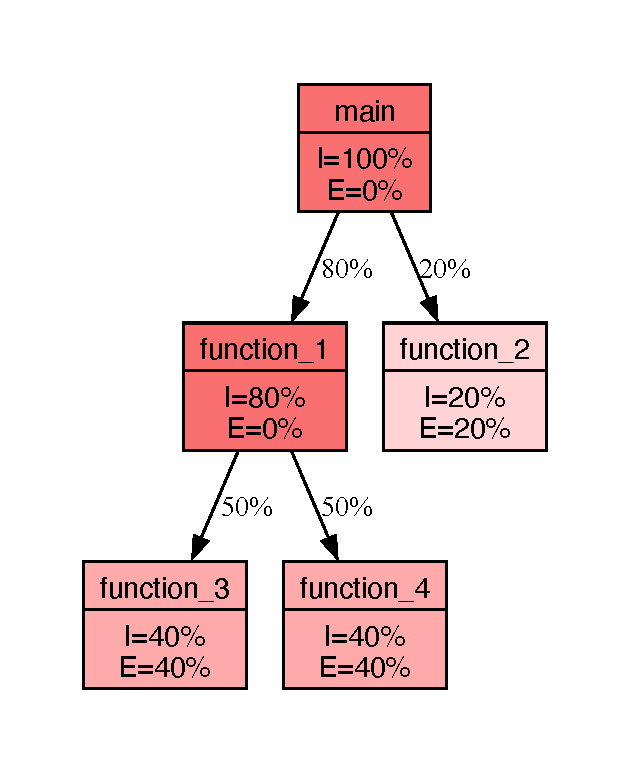
\includegraphics[page=1]{Bilder/pdf/profiler_output_example.pdf}
    \end{center}
    \caption{Beispielausgabe des HANA Profilers}\label{fig:beispielausgabe_hana_profiler}
\end{figure}


\chapter{Benchmarking-Konzept}
\section{Messung} % (fold)
\label{sec:Messung}
Um Messwerte sinnvoll miteinander vergleichen zu können, dürfen diese sich bis
auf einen Parameter nicht unterscheiden. Bei der Analyse, wie sich verschiedene
Modelle auf die Laufzeit der Optimierung von diesen auswirken, sind die Größe
und der Aufbau des Modells als Parameter denkbar. Der Aufbau, im folgenden auch
Art des Modells genannt, wird durch eine Funktion beschrieben, welche für einen
Parameter $n$ ein Modell der Größe $n$ erzeugt. $n$ ist dabei nicht zwingend
die Anzahl der Knoten im Modell, sondern könnte auch festlegen, wie
oft ein bestimmtes Muster in dem Modell wiederholt wurde.

Ist die Größe in einer Messreihe der veränderliche Parameter, muss der Aufbau
des Modells unveränderlich sein.
% section Messung (end)
\section{Testdaten} % (fold)
\label{sec:Testdaten}

% section Testdaten (end)

\chapter{Umsetzung}
\section{Implementation der neuen Methode}

\chapter{Verifikation}

\chapter{Fazit und Ausblick}


% ---- Literaturverzeichnis
\cleardoublepage
\renewcommand*{\chapterpagestyle}{plain}
\pagestyle{plain}
\pagenumbering{Roman}                   % Römische Seitenzahlen
\setcounter{page}{\numexpr\value{savepage}+1}
\printbibliography[title=Literaturverzeichnis]

% ---- Anhang
\appendix
%\clearpage
%\pagenumbering{Roman}  % römische Seitenzahlen für Anhang

\newpage
\end{document}
